% !TeX encoding = UTF-8
\section{Umsetzung}
\label{sec:Umsetzung}
Es gibt unterschiedliche Vorgehensweisen, einen RRT* zu bauen und neu zu verknüpfen. Besondere Bedeutung hat dabei, wie neu erzeugte Knoten dem Baum hinzugefügt werden. David Gödicke benutzte in seiner Bachelorarbeit zum Erreichen zweier Punkte innerhalb des Baumes Dubin curves \citep{Dubin61} beziehungsweise Reed Sheep curves \citep{reeds1990optimal}, sodass der neu hinzugefügte Knoten stets durch seinen Vater erreichbar war \citep{Goedicke18}. Leider war die Berechnung dadurch insgesamt zu aufwändig und langsam, was für Echtzeit-Szenarien im Straßenverkehr ein hartes Ausschlusskriterium ist, weshalb Goedicke diesen Ansatz nicht empfehlen konnte \citep[vergleiche][Kapitel 7]{Goedicke18}. \\
Daher entschloss ich mich, Varianten von RRT* zu untersuchen, bei denen das Auto direkt von Knoten zu Knoten fährt. Dadurch benötigt es nur eine Lenkeinstellung zwischen zwei Knoten und die Berechnung wird einfacher.\\
\begin{figure}
	\label{fig:reachable}
	\centering
	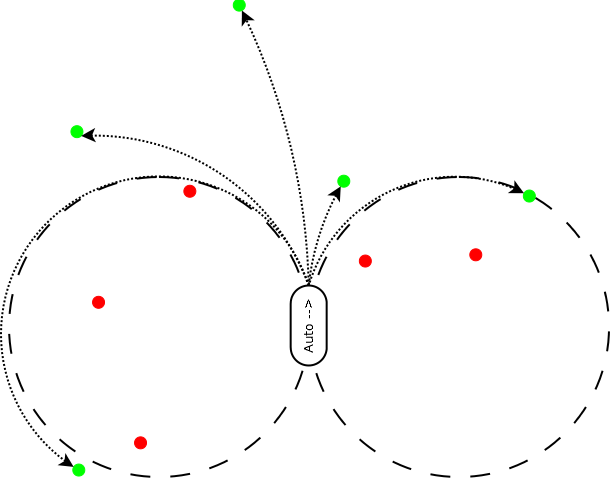
\includegraphics[scale=0.6]{Bilder/Erreichbarkeit_Punkte.png}
	\caption{Erreichbare und nicht erreichbare Punkte vom Auto aus}
\end{figure}
\subsection{Übersicht}
\label{sec:uebersicht}
Hier werden vier verschiedene Ansätze vorgestellt, mit deren Hilfe das Auto mit dem RRT* Algorithmus von der Startposition in den Zielbereich kommt.
\begin{enumerate}
\item Erster Ansatz: Nicht erreichbare Knoten werden dem Baum nicht hinzugefügt. Kostenfunktion berücksichtigt Lenkänderungen. Rewiring findet Rekursiv statt.
\item Zweiter Ansatz: Alle Knoten sind erreichbar, aber nur außerhalb der Wendekreise. Kostenfunktion berücksichtigt Lenkänderungen. [TODO: Rewiring?]
\item Dritter Ansatz: RRT* ohne Einschränkungen durchgeführt, das heißt alle Knoten sind gültig. Am Ende wird ein Pfad vom Ziel zum Startknoten erstellt, der abfahrbar ist.
\item Vierter Ansatz: Nicht erreichbare Knoten werden dem Baum nicht hinzugefügt. Kostenfunktion berücksichtigt Lenkänderungen. Rewiring wird nur bei dem Knoten mit der besten Kostenersparnis durchgeführt.
\end{enumerate}
Dabei müssen diese Ansätze folgende Bedingungen erfüllen: \\
\begin{enumerate}
\item Garantie der Abfahrbarkeit: Das Auto muss in der Lage sein, der berechneten Trajektorie zu folgen. Da das Auto die Punkte innerhalb der Wendekreise nicht erreichen kann(siehe \ref{fig:reachable}), muss sichergestellt werden dass diese Punkte nicht als Kindknoten gewählt werden können.
\item Geringe Kosten: Es muss nicht der optimale Pfad gefunden werden, aber er sollte zumindest asymptotisch optimal sein. 
\item Niedrige Berechnungsdauer: Da der Algorithmus mehrmals pro Sekunde ausgeführt werden soll, sind Ausführzeiten über 250 Millisekunden nicht tolerierbar. Bei Messungen der Ausführzeit muss jedoch auch die Wahl der Datenstruktur, Metrik und die Art der Implementierung berücksichtigt werden, da diese zusätzlich die Laufzeit verändern können.
\end{enumerate}
Die vier Ansätze werden anhand der obigen Kriterien untersucht und bewertet.

\subsection{Erster Ansatz}
Ziel ist es hier, nur Knoten hinzuzufügen, die vom jeweiligen Vaterknoten auch erreichbar sind. Um eine bessere Laufzeit zu erreichen, wurde schon bei der Suche des nächsten Nachbarn eine Vorauswahl getroffen und ein Großteil der nicht vom Baum erreichbare Knoten aussortiert. Bei der tatsächlichen Bestimmung des Vaterknotens werden dann mithilfe eines genaueren Mechanismus nur Knoten berücksichtigt, von denen aus der neu hinzugefügte Knoten erreicht werden kann. \\
Nach dem Setzen des Vaterknotens werden mit einer Kostenfunktion die Kosten berechnet, um diesen Knoten zu erreichen. Zum Schluss findet das Rewiring, das neu verknüpfen des Baumes, statt.
\subsubsection{Vorauswahl}
\label{sec:Vorauswahl}
Diese beinhaltete, bei der Erstellung des RRT* vom Auto nicht erreichbare Knoten gar nicht erst zuzulassen. Das Auto sollte also von einem Knoten zum nächsten mit nur einer Lenkeinstellung direkt fahren können. Dies sollte die Berechnungszeit stark verringern. \\
Zum Ausschluss der Knoten verwendete ich zuerst eine Heuristik: Ein nächster Nachbar N für einen neu hinzugefügten Knoten K kam nur dann in Frage, falls dieser den neu hinzugefügten Knoten K auch erreichen konnte. Dazu wurde die Ausrichtung des Autos im potenziellen Elternknoten N mit dem Richtungsvektor zwischen den beiden Knoten verglichen. Somit war K gültig, falls der Winkel zwischen der Ausrichtung von N und dem direktem Weg zum Knoten K (Richtungsvektor) einen bestimmten Wert $\gamma$ nicht überschritt.
\begin{figure}
\centering
\label{fig:fig4}
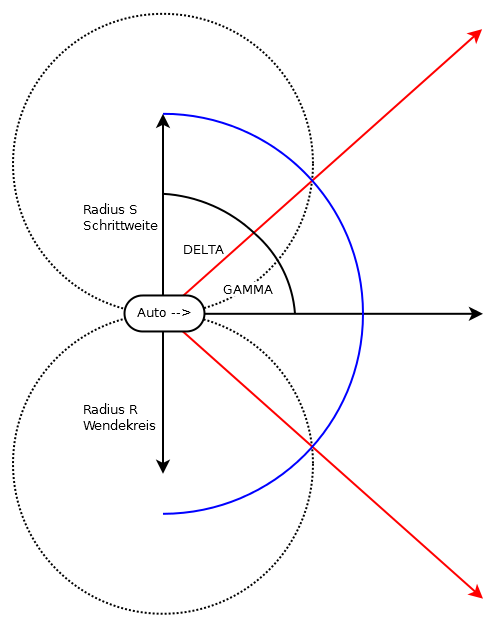
\includegraphics[scale=0.6]{Bilder/AusrichtungGrob.png} 
\caption{Bedeutung der Schrittweite und Radius für den Winkel Gamma}
\end{figure}
 $\gamma$ direkt zu berechnen war nicht ohne weiteres möglich, doch mit Hilfe des Kosinussatzes konnte der Winkel $\delta$ (siehe Abbildung ~\ref{fig:fig4}) berechnet werden. Dieser berechnet sich aus dem Radius $R$ des Wendekreises des Autos und der verwendeten Schrittweite, also dem maximalen Abstand zwischen zwei Knoten. \\
Der Knoten K wurde im ersten Schritt als gültig erkannt, wenn für die Differenz zum Winkel des Elternknoten galt: 
\begin{center}
$diff(K,N) <\gamma$ \\
$\gamma = 90^{\circ} - \delta$  \\
$\delta = arccos (\frac{Schrittweite}{2 \dot R})$  \\
\end{center}

Alle Knoten außerhalb dieses Winkels würden bei der Projektion im Wendekreis des Autos landen, wie in Abbildung \ref{fig:fig5} zu sehen. Diese Knoten(rot) wurden verworfen.\\
\subsubsection{Auswahl des Vaterknotens}
\label{sec:Auswahl}
Als nächster Schritt wird, wie in Kapitel \ref{RRT*} geschildert, der Knoten K an den nächsten (gültigen) Nachbarn N projiziert und der Vaterknoten bestimmt. Sollte der Knoten näher am Vaterknoten dran sein, als die Schrittweite ist, wird der Knoten nicht projiziert, da sonst alle Knoten zu ihrem Vaterknoten den gleichen Abstand hätten und bestimmte Bereiche somit nicht auf optimalen Weg erreichbar wären. Da innerhalb der Schrittweite durch den maximalen Lenkwinkel des Autos selbst die Knoten, die vom Winkel her gültig sind, nicht erreichbar sein können, ist eine zusätzliche Überprüfung für diese Knoten notwendig (siehe \ref{fig:fig5}). \\
Da der maximale Lenkwinkel eines Autos vorgegeben ist, hängt also die Erreichbarkeit des Knotens allein von der Schrittweite ab. Mit dieser kann auch vorgegeben werden, um wie viel Grad sich die Ausrichtung des Autos bei einem Schritt ändern darf und ob beispielsweise Kehren erlaubt sind. Dabei muss jedoch beachtet werden: Bei einer zu kleinen Schrittweite werden viele Knoten verworfen und es werden kaum enge Kurven möglich sein. Bei einer zu großen Schrittweite werden sehr kurvige Trajektorien entstehen, sodass z.B. Hinderniserkennung nicht mehr so einfach ist.
\begin{figure}
\centering
\label{fig:fig5}
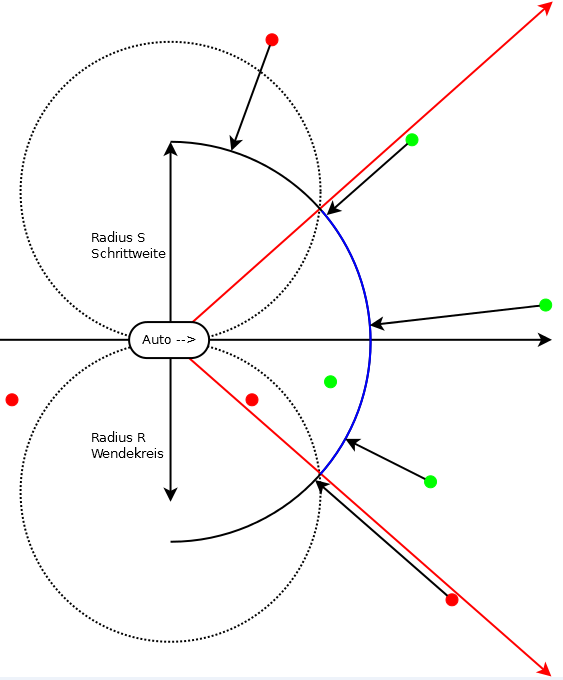
\includegraphics[scale=0.6]{Bilder/Projektion_der_Punkte.png} 
\caption{Projektion der Punkte auf Schrittweite}
\end{figure}
\subsubsection{Bestimmung des Vaterknotens}
Nachdem der Knoten an seinen nächsten Nachbarn projiziert wurde, wird nun aus allen nächsten Nachbarn innerhalb eines Radius R der mit den besten Kosten gewählt. Im Verfahren zur Bestimmung des nächsten Nachbarn, siehe \ref{sec:Vorauswahl}, wurden nicht beachtet, dass der neue Knoten innerhalb der Wendekreise des Autos liegen könnte. Es ist dem Auto aber nicht möglich, vom Vaterknoten N zum Knoten K zu fahren, wenn K im Wendekreis des Autos liegt. \\
Für jeden Knoten im Radius R wird geprüft, ob dieser Knoten unseren neuen Knoten K erreichen kann. Das wird ausgerechnet, indem vom potentiellen Vaterknoten N aus zwei Mittelpunkte der Wendekreise bestimmt werden. Wenn der Abstand von K zu diesen Mittelpunkten kleiner ist als der Radius der Wendekreise, liegt K im Wendekreis und ist nicht erreichbar. Damit kommt N als Nachbar nicht in Frage. Falls kein nächster Nachbar im Radius R den Knoten K erreichen kann, wird K verworfen. \\
Nachdem erfolgreich ein Vaterknoten bestimmt und dem neu hinzugefügtem Knoten K zugewiesen wurde, muss noch die Ausrichtung oder Orientierung bestimmt werden, die das Auto im Knoten K hat.
\subsubsection{Bestimmung der Orientierung}

\begin{figure}
\label{fig:fig8}
\centering
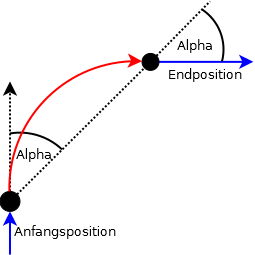
\includegraphics[scale=0.8]{Bilder/BerechnungOrientierung.png} 
\caption{Berechnung der Ausrichtung}
\end{figure}
Da das Auto im Vaterknoten N eine bestimmte Ausrichtung hat und mit nur einer Lenkeinstellung zum nächsten Knoten K gelangt, ist dort die Ausrichtung dadurch festgelegt und berechnet sich aus der Ausrichtung des Vaterknotens, Winkel $\theta$, und dem Winkel zwischen der Ausrichtung des Vaterknotens und dem Richtungsvektor von N nach K. Wie in der Zeichnung ~\ref{fig:fig8} zu sehen ist, berechnet sich die Ausrichtung $\omega$ des neuen Knotens K folgendermaßen:
\begin{center}
	$\theta + 2 \pi - 2*\alpha = \omega$
\end{center}

\subsubsection{Kostenfunktion}
\label{sec:Kosten}
Eine besondere Bedeutung zur Erzeugung einer "guten" Trajektorie kommt der Kostenfunktion zu. Diese sorgt nicht nur dafür, welcher Knoten als Vaterknoten ausgewählt wird, sondern spielt auch beim Neuverknüpfen des Baumes eine Rolle.Somit kann mithilfe der Kostenfunktion für besonders gut abfahrbare oder besonders kurze Pfade gesorgt werden. \\
Da durch die Orientierung des Vaterknotens die Orientierung des Kindknotens bereits festgelegt ist (siehe Abbildung ~\ref{fig:fig8}, können aus eigentlich geraden Strecken sehr ungünstige Pfade entstehen.\\
 In Abbildung ~\ref{fig:fig5} wird als Kostenfunktion der euklidische Abstand benutzt. Knoten C wählt aus B1 und B2 den nächsten Nachbarn aus, das ist B2. Leider entsteht dadurch eine sehr kurvige Route, bei der vom fast maximalem Lenkeinschlag nach rechts auf den maximalen Lenkeinschlag der anderen Seite gewechselt werden muss. Neben Nachteilen des Komforts, der Sicherheit und längerem Weg wird auch die Ungenauigkeit höher. Anfangs wurde angenommen, dass der Lenkwinkel sich sofort ändern kann. Während bei kleinen Änderungen diese Annahme nur für kleine Fehler sorgt, sind die Auswirkungen bei solch starken Änderungen deutlicher spürbar.


\begin{figure}[htb]
  \label{fig:fig6}  
    \centering
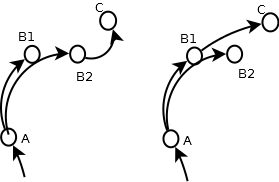
\includegraphics[scale=1]{Bilder/Gute_schlechte_funktion.png} 
\caption{Euklidische Kostenfunktion (rechts) gegenüber der erweiterten Kostenfunktion (links)}
\end{figure}


In Abbildung ~\ref{fig:fig9} hingegen wurde eine bessere Kostenfunktion gewählt, sodass über B1 gehend ein effizienterer, kürzerer Pfad entsteht. Die Kostenfunktion muss dabei die Ausrichtung des Autos beim Vaterknoten N berücksichtigen. \\
Es wurde eine Kombination aus dem euklidischem Abstand und der Winkeldifferenz der Knoten K und N zur Kostenberechnung zu benutzen. Die Kosten berechnen sich dann wie folgt: 
\begin{center}
$cost(K) = cost(N) +eukl. Abstand(K,N) * (1+Winkeldifferenz)$
\end{center} 
Bei einer geraden Strecke wird lediglich der euklidische Abstand als Kosten aufsummiert, bei einer Kehre von 180$^{\circ}$ bis zum vierfachen der euklidischen Kosten (Winkeldifferenz $\pi$ +1).\\
Nachteil dieser Kostenfunktion ist, dass nicht berücksichtigt wird, dass starke Kurven weniger schlimm sind auf größerer Strecke. Mit anderen Worten, das Fahren genau auf den minimalen Wendekreisen ist meist weniger angenehm beziehungsweise optimal als das Fahren auf weiten Kreisen, auch wenn beide Pfade die gleiche Winkeldifferenz haben. Das Problem hierbei ist, dass ein kleinerer Kreis geringere euklidische Kosten hat und demzufolge gegenüber dem größeren Kreis bevorzugt wird. Eine andere Möglichkeit wäre auch, die tatsächliche zu fahrende Strecke des Autos zu benutzen anstatt des euklidischen Abstands und dadurch effizientere Pfade zu bevorzugen. Eine andere Möglichkeit ist, zu harte Richtungsänderungen zu bestrafen und kleine $ \Delta \theta$ zu bevorzugen. \\
\subsubsection{Rewiring}
Der Knoten K wurde neu in den Baum hinzugefügt. Nun wird überprüft, ob bereits vorhandene Knoten besser erreichbar sind, wenn der Weg über K gewählt wird(siehe \ref{sec:rewiring}).
Dazu werden zunächst im Radius R alle in Frage kommenden Nachbarn ausgewählt. Diese Menge wird hier als M bezeichnet. Von M aussortiert werden alle, die entweder vom Knoten K aus nicht erreichbar sind (gleiche Überprüfungen wie in \ref{sec:Auswahl}) oder aber bei denen K keine Verbesserung bewirkt, also die Kosten - über den Knoten K - gleich oder höher sind). \\
\begin{figure}
\centering
\label{fig:rewiringNodeInvalid}
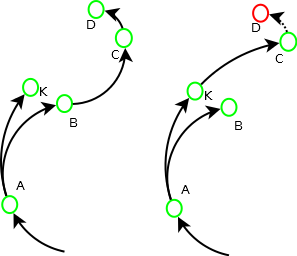
\includegraphics[scale=0.7]{Bilder/Rewiring_ungueltige_knoten.png} 
\caption{Knoten K wird neuer Nachbar von C - Knoten D kann nicht mehr erreicht werden}
\end{figure}

Wenn man allen in M enthaltenen Knoten einfach K als Vater hinzufügen würde, müsste jeweils die Orientierung der Knoten in M, der Winkel $\theta$, geändert werden. Das Auto gelangt auf anderem Wege zu diesen Knoten und hat somit eine andere Ausrichtung als vorher. Allerdings kann es dadurch vorkommen, dass wenn der Knoten $C \in M$ eine neue Orientierung hat, Kinder von C nicht mehr durch C erreichbar sind (siehe \ref{fig:rewiringNodeInvalid}). Deshalb wird, anstatt die Orientierung zu ändern, einfach ein neuer Knoten hinzugefügt, der zwar die gleicher Koordinaten hat wie C, aber eine andere Orientierung. Dies wird mit allen von K erreichbaren Knoten durchgeführt. Alle somit zum Baum neu hinzugefügten Knoten sind durch K besser erreichbar. Dadurch werden allerdings keine Pfade verbessert, was eine Voraussetzung für die in \ref{sec:rrt*} genannte asymptotische Optimalität ist.\\
Die einzige vollständige Maßnahme wäre, für jeden so neu hinzugefügten Knoten ebenfalls das Rewiring durchzuführen, da ein durch diesen Knoten andere eventuell durch bessere Pfade erreichbar ist. Dadurch braucht man jedoch sehr viel Zeit, da der ganze Baum z.T. mehrfach neu verknüpft wird. Im schlechtesten Fall wäre die Laufzeit dabei exponentiell, da jeder Knoten alle seine Nachbarn neu verknüpfen könnte.
\subsubsection{Bewertung}
Leider kann diese Herangehensweise nur zwei von den drei geforderten Anforderungen erreichen. Die Abfahrbarkeit der Trajektorie ist in jedem Fall gewährleistet. Die asymptotische Optimalität kann jedoch nur gewährleistet werden, wenn das Rewiring komplett durch den ganzen Baum rekursiv, das heißt auf jeden durch das Rewiring neu hinzugefügten Knoten, angewendet wird. Dadurch entstehen exponentielle Laufzeiten, sodass der Aufbau des Baumes mehrere Sekunden in Anspruch nimmt, was auch nach Optmierung des Codes und der Datenstruktur zu viel ist. [TODO Messwerte einfügen]\\
Deshalb ist dieser Ansatz für den produktiven Einsatz nicht geeignet.

\subsection{Zweiter Ansatz}
Auf dem ersten Ansatz aufbauend wurde der zweite entwickelt. Das Problem des ersten war, dass das Rewiring nicht richtig durchgeführt werden konnte, weil sonst Knoten ungültig werden. \\
Theoretisch kann aber ein Auto mit nur einer Lenkeinstellung alle Punkte außerhalb der Wendekreise erreichen. Das Problem der Nichterreichbarkeit könnte also dadurch behoben werden, dass nur Knoten in einem bestimmten Abstand - so dass sie nicht innerhalb der Wendekreise sind -als Vaterknoten erlaubt sind.\\
\begin{figure}
\centering
\label{fig:zweiteransatz}
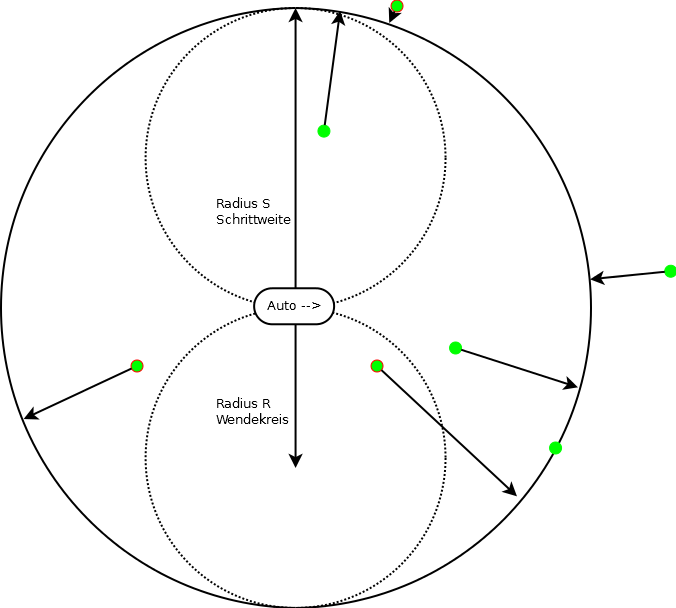
\includegraphics[scale=0.5]{Bilder/Zweiter_Ansatz_Projektion.png} 
\caption{Je nach dem, wo der Punkt erzeugt wurde, wird er auf Schrittweite verschoben}
\end{figure}
\subsubsection{Veränderungen}
Die im ersten Ansatz beschriebene Vorauswahl fällt weg, da erstmal jeder Knoten erreichbar ist. Bei der Projektion an den nächsten Nachbarn muss darauf geachtet werden, dass der Projektionsabstand größer als der Durchmesser der Wendekreise ist. Die Auswahl des Vaterknotens findet nur außerhalb eines bestimmten Kreises statt, da im Inneren je nach Ausrichtung des Autos nicht alle Punkte erreichbar sind. Der Radius des Kreises entspricht dem Durchmesser der Wendekreise des Autos (siehe \ref{fig:zweiteransatz}).\\
Dadurch gibt es keine ungültigen Punkte in der Trajektorie. Wenn das Rewiring durchgeführt wird, wird in allen Knoten, die durch den neu hinzugefügten Knoten besser erreichbar sind, die Ausrichtung neu berechnet, wie in \ref{sec:Rewiring} beschrieben. Als Kostenfunktion kann nur der euklidische Abstand verwendet werden, da die Ausrichtung veränderlich ist. \\
Die Abstände zwischen zwei so verbundenen Knoten sind sehr groß, was die Vermeidung von Hindernissen schwierig macht.\\
Auch können kurvige Trajektorien durch z.B. eine Kostenfunktion nicht vermieden werden, da die Kostenfunktion dazu die Ausrichtungen in einem Knoten benötigen würde, um die Änderung der Orientierung zu bestimmen. Diese Ausrichtungen können zwar bestimmt werde, ändern sich jedoch mit jeder Neuverknüpfung. Alle Kosten jedes Mal neu zu berechnen, würde mit O(n) viel zu lange dauern.\\
\subsubsection{Bewertung}
Wie beim ersten Ansatz ist die entstehende Trajektorie vom Auto abfahrbar, hat also keine unerreichbaren Knoten. Die Geschwindigkeit des Algorithmus hat sich im Gegensatz zum ersten Knoten stark verbessert und für die Rewiring Operation wird nur noch O(log n) Zeit benötigt. \\
Die Pfade können zwar durch das Rewiring optimiert werden, jedoch entstehen große Herausforderungen bei der Hindernisvermeidung. Außerdem können kleine Zielbereiche nur über Umwege erreicht werden, da sie sonst aufgrund der Schrittweite einfach übersprungen werden. Ein weiterer Nachteil ist, dass kurvige Trajektorien nicht aktiv vermieden werden, da die Kostenfunktion nur auf den Koordinaten der Knoten basieren kann. Somit sind beim Auto auf dem Weg zum Ziel Schlangenlinien zu erwarten und der Pfad ist in diesem Sinne nicht optimal [TODO durch Testergebnisse beweisen] 

\subsection{Dritter Ansatz}
Bei diesem Ansatz soll erst im Nachhinein ein abfahrbarer Pfad erzeugt werden. Dazu wird der RRT* Algorithmus ohne Berücksichtigung der Ausrichtung $\theta$ ausgeführt. Dadurch das keine Einschränkungen gemacht werden, terminiert der Algorithmus schnell. Zur Berechnung der Kosten eines jeden Knoten wird eine Kostenfunktion c(K) verwendet. Sei K ein Knoten und V der Vater dieses Knotens: 
$c(K) = c(V) + euklid. dist(K,V)$   \\
\subsubsection{Erzeugung der Trajektorie}
Es wird der Zielknoten Z ausgewählt. Für diesen Knoten Z wird die Menge M aller Knoten in einem Kreis um Z gebildet.  Aus der Menge M wird der Vaterknoten V bestimmt, dessen Gesamtkosten am geringsten ist. Dabei wird zur Berechnung der Gesamtkosten auch die Änderung der Ausrichtung, um zu diesem Zielknoten zu gelangen, berücksichtigt, ähnlich wie in der Kostenfunktion des ersten Ansatzes. \\
Nach einer Laufzeit von maximal O(n log n) ist der Startknoten erreicht. Dadurch, dass vom Zielknoten aus gestartet wurde, kann es sein, dass das Auto vom Startknoten aus den ersten Knoten der Trajektorie gar nicht oder nicht mit der richtigen Orientierung erreichen kann. Deshalb werden für den ersten Schritt Dubins curves verwendet, mit denen das Auto einen beliebigen Punkt mit beliebiger Ausrichtung erreichen kann. Nach diesem ersten Schritt kann das Auto jeden Knoten mit nur einer Lenkeinstellung erreichen. \\

\subsubsection{Bewertung}
Durch RRT* und die Kostenfunktionen wird durch diesen Algorithmus nicht nur eine gültige Trajektorie erzeugt, sondern auch eine, bei der unnötige Kurven vermieden werden. Die Laufzeit liegt mit O(n log n) in einem vertretbaren Rahmen. \\
Bei der Problembeschreibung (\ref{sec:uebersicht}) wurde festgesetzt, dass der Algorithmus mindestens vier Mal pro Sekunde durchgeführt werden soll. Es ist zu erwarten, dass das Auto mehr als 250 Millisekunden braucht, um auf den vorgeschlagenen Pfad zu kommen, also den ersten Knoten mit korrekter Ausrichtung zu erreichen. Nach 250 Millisekunden wird jedoch ein komplett neuer Baum aufgebaut, sodass alle aufwändigen Berechnungen, um eine gute Trajektorie zu erstellen, umsonst waren. Somit wird das Auto stets nur den ersten Teil mit den Dubins curves abfahren, was den ganzen Sinn des Algorithmus in Frage stellt. \\
Dieser Ansatz ist also so ausgeführt nicht sinnvoll. Eine Möglichkeit wäre, den Baum wiederzuverwenden und somit auch die erzeugte Trajektorie. Allerdings muss dafür die Datenstruktur das sogenannte Prunning, also Abtrennen von Ästen des Baumes, unterstützen, um keine nicht erreichbaren Knoten und deren Kinder zu verwenden. Ohne diese Datenstruktur ist ein weiteres Vertiefen in diesen Ansatz nicht sinnvoll.

\subsection{Vierter Ansatz}
Nach dem erfolglosen Beschäftigen mit dem dritten Ansatz wurde der Fokus wieder mehr auf den ursprünglichen Ansatz und das Rewiring gelegt. Ziel war es nun, anstelle des rekursiven Rewiring eine andere, schnellere und trotzdem asymptotisch optimale Lösung zu finden. \\
\subsubsection{Rewiring}
Das Problem war, das mit jedem Rewiring eine große Anzahl an Knoten hinzugefügt wurden, auch wenn diese zum Teil nur marginale Verbesserungen boten, und dass jeder so hinzugefügte Knoten jeweils auch eine Rewiring Operation auslöste.\\
Anstatt für jeden Knoten, der durch das Rewiring besser erreichbar ist, einen neuen Knoten hinzuzufügen (\ref{sec:rewiring}) wird nur dem Knoten K ein neuer Knoten hinzugefügt, bei dem die Auswirkungen am größten sind. Dazu werden die Kosten von K mit den Kosten verglichen, die ein neu hinzugefügter Knoten an der Position von K hätte. Dies wird mit allen Knoten im Radius R durchgeführt und beim Paar mit der größten Differenz wird tatsächlich ein neuer Knoten hinzugefügt. \\
\begin{figure}
\label{fig:rewiring4}
\centering
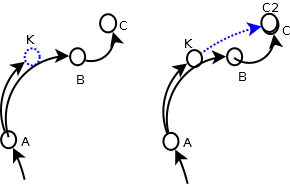
\includegraphics[scale=1]{Bilder/Rewiring.png} 
\caption{Rewiring}
\end{figure}
Das Ganze wird verdeutlicht an einem Beispiel in \ref{fig:rewiring4}. Hier wird Knoten K neu hinzugefügt. In der Liste der Erreichbaren Knoten stehen B und C. Weil bei B keine Kostenverbesserung stattfindet, ist bei C die Differenz zwischen alten Kosten und Kosten eines neuen Knotens an dieser Position am geringsten. Deshalb wird nun mit den gleichen Koordinaten wie C ein neuer Knoten $C_2$ erstellt. Nun wird überprüft ob $C_2$ weitere Knoten verbessern kann. Da dies nicht der Fall ist, endet das Rewiring und der Algorithmus fährt normal fort.\\
Das Rewiring wird so lange durchgeführt, bis kein Knoten mehr gefunden wird, dessen Kosten durch Neuverknüpfung geringer wären. Bei einer geeigneten Wahl der Schrittweite (nicht zu groß, \ref{sec:Auswahl}) kann dies relativ schnell eintreten, weil gar nicht so viele in Frage kommen. \\
Damit nicht immer beim gleichen Knoten das Rewiring durchgeführt wird, weil die Kostendifferenz bei diesem Knoten immer am höchsten ist, werden im alten Knoten auch die Kosten des neuen Knotens, der die gleichen Koordinaten hat, gespeichert. Beim Rewiring wird ein Knoten mit diesen Koordinaten nur dann hinzugefügt, falls dessen Kosten geringer sind als die aller Knoten mit diesen Koordinaten.

\subsubsection{Bewertung}
Der Vorteil dieses Mechanismus ist, dass mögliche Optimierungen schnell durch den Baum wandern und keine Knoten ungültig werden. Außerdem müssen nicht so viele randomisierte Punkte erzeut werden, was der Laufzeit zu Gute kommt.\\
 Nachteile sind allerdings eine geringere Anzahl von räumlich verteilten Punkten (es liegen Punkte \glqq übereinander\grqq). Zudem kann dieses Verfahren viel Zeit beanspruchen, ohne viel Effekt zu haben, wenn bereits viele Punkte im Baum existieren und Bereiche weit abseits der Zielregion neu verknüpft werden. \\
 Abschließend kann man sagen, dass von allen vier Ansätzen dieser der vielversprechenste ist. Es werden nicht nur gültige Pfade gefunden, sondern auch optimale, die in angemessener Zeit berechnet werden können[TODO Testergebnisse/Beweis].


\subsection{Dokumentation der Durchführung und Erkenntnisse daraus}
[TODO - mit rein nehmen oder rauslassen?] 



\subsubsection{Beschreibung erkannter Schwierigkeiten und Fehler}
[TODO - mit rein nehmen oder rauslassen?] 
Im Nachhinein betrachtet habe ich viele methodische Fehler gemacht. Zuerst wurde das Problem begutachtet, dann analysiert und ein Lösungsvorschlag gemacht. Dieser Lösungsvorschlag wurde aber nicht bis ins Detail auf die Machbarkeit überprüft, sondern ich habe versucht Teile davon direkt umzusetzen. Insgesamt habe ich den Aufwand dieser ersten Umsetzung stark unterschätzt. Ich musste mich sowohl in eine unbekannte Programmiersprache (C++) und in ein weitgehend unbekanntes Framework (ROS) einarbeiten. Besonders bei Letzterem kommunizierte ich zu wenig mit den wissenschaftlichen Mitarbeitern des Arbeitsbereichs. Somit verschlang schon die Einarbeitung und der Entwurf eines Prototypens sehr viel Zeit, ohne zu befriedigenden Ergebnissen zu kommen. Doch auch technische Probleme und Schwierigkeiten mit der vorhandenen Infrastruktur nahmen viel Zeit in Anspruch.\\
Als der Lösungsansatz endlich vollständig implementiert wurde, ist aufgefallen, dass dieser an einigen Stellen nicht funktionierte. Deshalb wurde versucht, den Lösungsansatz zu verbessern und diese verbesserte Lösung zu implementieren. Da ich zu wenig dabei mit anderen Mitarbeitern kommunizierte, hatte auch die verbesserten Lösungen Fehler, sodass ich mich oft in Sackgassen wiederfand. \\
Besonders am Anfang war, kombiniert mit häufigem Scheitern an Abhängigkeiten und Installationsproblemen, die dadurch resultierende Motivationslosigkeit ein großes Problem, was dann auch schnell zu einem Zeitproblem wurde. 

\subsubsection{Verbesserungen in der Arbeitsweise}
Ich habe festgestellt, dass sowohl detallierte Planung (was mache ich an jedem Tag der nächsten Woche) als auch globale Planung (welche Artefakte sollen bis wann fertig gestellt werden?) sehr wichtig sind und gründlich mit Sorgfalt durchgeführt werden sollten. \\
Bei Fehlschlägen ist es wichtig, sich - je nach Problem - an andere zu wenden, wenn man selbst das Problem nicht ohne weiteres lösen kann. Dies ist vor allem bei wiederkehrenden Problemen wie beim Aufsetzen von Software der Fall, deren Lösung längst bekannt ist. \\
Es ist sehr wichtig, sich über den theoretischen Ansatz und dessen Machbarkeit intensiv Gedanken zu machen, dabei auch verschiedene wissenschaftliche Quellen zu untersuchen. Stellt sich heraus, dass der eigene Ansatz nicht umsetzbar ist, sollte ein Gespräch mit dem Betreuer vereinbart werden, um Lösungen zu besprechen, bevor eigene fehlerhafte Ansätze implementiert werden. \\
Bei den Gesprächen mit den Mitarbeitern und Betreuern ist es wichtig, ein klares Anliegen bzw. eine klare Problemstellung zu haben und dies angemessen zu formulieren.
